% Options for packages loaded elsewhere
\PassOptionsToPackage{unicode}{hyperref}
\PassOptionsToPackage{hyphens}{url}
%
\documentclass[
]{article}
\title{hw8}
\author{}
\date{\vspace{-2.5em}}

\usepackage{amsmath,amssymb}
\usepackage{lmodern}
\usepackage{iftex}
\ifPDFTeX
  \usepackage[T1]{fontenc}
  \usepackage[utf8]{inputenc}
  \usepackage{textcomp} % provide euro and other symbols
\else % if luatex or xetex
  \usepackage{unicode-math}
  \defaultfontfeatures{Scale=MatchLowercase}
  \defaultfontfeatures[\rmfamily]{Ligatures=TeX,Scale=1}
\fi
% Use upquote if available, for straight quotes in verbatim environments
\IfFileExists{upquote.sty}{\usepackage{upquote}}{}
\IfFileExists{microtype.sty}{% use microtype if available
  \usepackage[]{microtype}
  \UseMicrotypeSet[protrusion]{basicmath} % disable protrusion for tt fonts
}{}
\makeatletter
\@ifundefined{KOMAClassName}{% if non-KOMA class
  \IfFileExists{parskip.sty}{%
    \usepackage{parskip}
  }{% else
    \setlength{\parindent}{0pt}
    \setlength{\parskip}{6pt plus 2pt minus 1pt}}
}{% if KOMA class
  \KOMAoptions{parskip=half}}
\makeatother
\usepackage{xcolor}
\IfFileExists{xurl.sty}{\usepackage{xurl}}{} % add URL line breaks if available
\IfFileExists{bookmark.sty}{\usepackage{bookmark}}{\usepackage{hyperref}}
\hypersetup{
  pdftitle={hw8},
  hidelinks,
  pdfcreator={LaTeX via pandoc}}
\urlstyle{same} % disable monospaced font for URLs
\usepackage[margin=1in]{geometry}
\usepackage{color}
\usepackage{fancyvrb}
\newcommand{\VerbBar}{|}
\newcommand{\VERB}{\Verb[commandchars=\\\{\}]}
\DefineVerbatimEnvironment{Highlighting}{Verbatim}{commandchars=\\\{\}}
% Add ',fontsize=\small' for more characters per line
\usepackage{framed}
\definecolor{shadecolor}{RGB}{248,248,248}
\newenvironment{Shaded}{\begin{snugshade}}{\end{snugshade}}
\newcommand{\AlertTok}[1]{\textcolor[rgb]{0.94,0.16,0.16}{#1}}
\newcommand{\AnnotationTok}[1]{\textcolor[rgb]{0.56,0.35,0.01}{\textbf{\textit{#1}}}}
\newcommand{\AttributeTok}[1]{\textcolor[rgb]{0.77,0.63,0.00}{#1}}
\newcommand{\BaseNTok}[1]{\textcolor[rgb]{0.00,0.00,0.81}{#1}}
\newcommand{\BuiltInTok}[1]{#1}
\newcommand{\CharTok}[1]{\textcolor[rgb]{0.31,0.60,0.02}{#1}}
\newcommand{\CommentTok}[1]{\textcolor[rgb]{0.56,0.35,0.01}{\textit{#1}}}
\newcommand{\CommentVarTok}[1]{\textcolor[rgb]{0.56,0.35,0.01}{\textbf{\textit{#1}}}}
\newcommand{\ConstantTok}[1]{\textcolor[rgb]{0.00,0.00,0.00}{#1}}
\newcommand{\ControlFlowTok}[1]{\textcolor[rgb]{0.13,0.29,0.53}{\textbf{#1}}}
\newcommand{\DataTypeTok}[1]{\textcolor[rgb]{0.13,0.29,0.53}{#1}}
\newcommand{\DecValTok}[1]{\textcolor[rgb]{0.00,0.00,0.81}{#1}}
\newcommand{\DocumentationTok}[1]{\textcolor[rgb]{0.56,0.35,0.01}{\textbf{\textit{#1}}}}
\newcommand{\ErrorTok}[1]{\textcolor[rgb]{0.64,0.00,0.00}{\textbf{#1}}}
\newcommand{\ExtensionTok}[1]{#1}
\newcommand{\FloatTok}[1]{\textcolor[rgb]{0.00,0.00,0.81}{#1}}
\newcommand{\FunctionTok}[1]{\textcolor[rgb]{0.00,0.00,0.00}{#1}}
\newcommand{\ImportTok}[1]{#1}
\newcommand{\InformationTok}[1]{\textcolor[rgb]{0.56,0.35,0.01}{\textbf{\textit{#1}}}}
\newcommand{\KeywordTok}[1]{\textcolor[rgb]{0.13,0.29,0.53}{\textbf{#1}}}
\newcommand{\NormalTok}[1]{#1}
\newcommand{\OperatorTok}[1]{\textcolor[rgb]{0.81,0.36,0.00}{\textbf{#1}}}
\newcommand{\OtherTok}[1]{\textcolor[rgb]{0.56,0.35,0.01}{#1}}
\newcommand{\PreprocessorTok}[1]{\textcolor[rgb]{0.56,0.35,0.01}{\textit{#1}}}
\newcommand{\RegionMarkerTok}[1]{#1}
\newcommand{\SpecialCharTok}[1]{\textcolor[rgb]{0.00,0.00,0.00}{#1}}
\newcommand{\SpecialStringTok}[1]{\textcolor[rgb]{0.31,0.60,0.02}{#1}}
\newcommand{\StringTok}[1]{\textcolor[rgb]{0.31,0.60,0.02}{#1}}
\newcommand{\VariableTok}[1]{\textcolor[rgb]{0.00,0.00,0.00}{#1}}
\newcommand{\VerbatimStringTok}[1]{\textcolor[rgb]{0.31,0.60,0.02}{#1}}
\newcommand{\WarningTok}[1]{\textcolor[rgb]{0.56,0.35,0.01}{\textbf{\textit{#1}}}}
\usepackage{graphicx}
\makeatletter
\def\maxwidth{\ifdim\Gin@nat@width>\linewidth\linewidth\else\Gin@nat@width\fi}
\def\maxheight{\ifdim\Gin@nat@height>\textheight\textheight\else\Gin@nat@height\fi}
\makeatother
% Scale images if necessary, so that they will not overflow the page
% margins by default, and it is still possible to overwrite the defaults
% using explicit options in \includegraphics[width, height, ...]{}
\setkeys{Gin}{width=\maxwidth,height=\maxheight,keepaspectratio}
% Set default figure placement to htbp
\makeatletter
\def\fps@figure{htbp}
\makeatother
\setlength{\emergencystretch}{3em} % prevent overfull lines
\providecommand{\tightlist}{%
  \setlength{\itemsep}{0pt}\setlength{\parskip}{0pt}}
\setcounter{secnumdepth}{-\maxdimen} % remove section numbering
\ifLuaTeX
  \usepackage{selnolig}  % disable illegal ligatures
\fi

\begin{document}
\maketitle

\hypertarget{section}{%
\section{1)}\label{section}}

\begin{enumerate}
\def\labelenumi{\alph{enumi}.}
\tightlist
\item
  use the method for the log-rank test to find the sample size needed.
  Assume that all patients who have not relapsed by 180 days will be
  censored at that point, and none will be censored before that point.
\end{enumerate}

\hypertarget{we-need-456-people}{%
\section{We need 456 people}\label{we-need-456-people}}

\begin{Shaded}
\begin{Highlighting}[]
\FunctionTok{library}\NormalTok{(asaur)}
\FunctionTok{library}\NormalTok{(survival)}
\NormalTok{LogRankDeaths }\OtherTok{\textless{}{-}} \ControlFlowTok{function}\NormalTok{(Delta, p, alpha, pwr) \{}
\NormalTok{  z.alpha }\OtherTok{\textless{}{-}} \FunctionTok{qnorm}\NormalTok{(alpha, }\AttributeTok{lower.tail =} \ConstantTok{FALSE}\NormalTok{)}
\NormalTok{  z.beta }\OtherTok{\textless{}{-}} \FunctionTok{qnorm}\NormalTok{(}\DecValTok{1} \SpecialCharTok{{-}}\NormalTok{ pwr, }\AttributeTok{lower.tail =} \ConstantTok{FALSE}\NormalTok{)}
\NormalTok{  num }\OtherTok{\textless{}{-}}\NormalTok{ (z.alpha }\SpecialCharTok{+}\NormalTok{ z.beta) }\SpecialCharTok{\^{}} \DecValTok{2}
\NormalTok{  denom }\OtherTok{\textless{}{-}}\NormalTok{ p}\SpecialCharTok{*}\NormalTok{(}\DecValTok{1}\SpecialCharTok{{-}}\NormalTok{p)}\SpecialCharTok{*}\NormalTok{(}\FunctionTok{log}\NormalTok{(Delta)) }\SpecialCharTok{\^{}} \DecValTok{2}
\NormalTok{  dd }\OtherTok{\textless{}{-}}\NormalTok{ num }\SpecialCharTok{/}\NormalTok{ denom}
\NormalTok{  dd}
\NormalTok{\}}

\FunctionTok{LogRankDeaths}\NormalTok{(}\FloatTok{0.7}\NormalTok{, }\FloatTok{0.5}\NormalTok{, }\FloatTok{0.05}\NormalTok{, }\FloatTok{0.9}\NormalTok{)}
\end{Highlighting}
\end{Shaded}

\begin{verbatim}
## [1] 269.2674
\end{verbatim}

\begin{Shaded}
\begin{Highlighting}[]
\NormalTok{fit\_survfit  }\OtherTok{=} \FunctionTok{survfit}\NormalTok{(}\FunctionTok{Surv}\NormalTok{(ttr, relapse) }\SpecialCharTok{\textasciitilde{}}\NormalTok{ grp, }\AttributeTok{data =}\NormalTok{ pharmacoSmoking)}
\FunctionTok{summary}\NormalTok{(fit\_survfit)}
\end{Highlighting}
\end{Shaded}

\begin{verbatim}
## Call: survfit(formula = Surv(ttr, relapse) ~ grp, data = pharmacoSmoking)
## 
##                 grp=combination 
##  time n.risk n.event survival std.err lower 95% CI upper 95% CI
##     0     61       4    0.934  0.0317        0.874        0.999
##     2     57       3    0.885  0.0408        0.809        0.969
##     4     54       1    0.869  0.0432        0.788        0.958
##     5     53       2    0.836  0.0474        0.748        0.934
##     8     51       2    0.803  0.0509        0.709        0.909
##    10     49       1    0.787  0.0524        0.691        0.897
##    12     48       1    0.770  0.0538        0.672        0.884
##    14     47       1    0.754  0.0551        0.653        0.870
##    15     46       2    0.721  0.0574        0.617        0.843
##    16     44       1    0.705  0.0584        0.599        0.829
##    20     43       1    0.689  0.0593        0.582        0.815
##    21     42       1    0.672  0.0601        0.564        0.801
##    30     41       2    0.639  0.0615        0.530        0.772
##    42     39       1    0.623  0.0621        0.512        0.757
##    50     38       1    0.607  0.0625        0.496        0.742
##    56     37       2    0.574  0.0633        0.462        0.712
##    60     35       2    0.541  0.0638        0.429        0.682
##    63     33       2    0.508  0.0640        0.397        0.650
##    65     31       1    0.492  0.0640        0.381        0.635
##    75     30       1    0.475  0.0639        0.365        0.619
##   110     29       1    0.459  0.0638        0.350        0.603
##   140     28       3    0.410  0.0630        0.303        0.554
##   170     25       1    0.393  0.0625        0.288        0.537
## 
##                 grp=patchOnly 
##  time n.risk n.event survival std.err lower 95% CI upper 95% CI
##     0     64       8    0.875  0.0413        0.798        0.960
##     1     56       5    0.797  0.0503        0.704        0.902
##     2     51       3    0.750  0.0541        0.651        0.864
##     3     48       1    0.734  0.0552        0.634        0.851
##     4     47       2    0.703  0.0571        0.600        0.824
##     6     45       1    0.688  0.0579        0.583        0.811
##     7     44       1    0.672  0.0587        0.566        0.797
##     8     43       1    0.656  0.0594        0.550        0.784
##    12     42       1    0.641  0.0600        0.533        0.770
##    14     41       6    0.547  0.0622        0.438        0.684
##    15     35       2    0.516  0.0625        0.407        0.654
##    21     33       1    0.500  0.0625        0.391        0.639
##    25     32       1    0.484  0.0625        0.376        0.624
##    28     31       3    0.438  0.0620        0.331        0.578
##    30     28       1    0.422  0.0617        0.317        0.562
##    40     27       1    0.406  0.0614        0.302        0.546
##    45     26       1    0.391  0.0610        0.288        0.530
##    49     25       1    0.375  0.0605        0.273        0.515
##    56     24       3    0.328  0.0587        0.231        0.466
##    77     21       2    0.297  0.0571        0.204        0.433
##    80     19       1    0.281  0.0562        0.190        0.416
##    84     18       1    0.266  0.0552        0.177        0.399
##   100     17       1    0.250  0.0541        0.164        0.382
##   105     16       1    0.234  0.0530        0.151        0.365
##   140     15       1    0.219  0.0517        0.138        0.348
##   155     14       1    0.203  0.0503        0.125        0.330
##   170     13       1    0.188  0.0488        0.113        0.312
\end{verbatim}

\begin{Shaded}
\begin{Highlighting}[]
\FunctionTok{plot}\NormalTok{(fit\_survfit, }\AttributeTok{col =} \FunctionTok{c}\NormalTok{(}\StringTok{"red"}\NormalTok{,}\StringTok{"blue"}\NormalTok{))}
\end{Highlighting}
\end{Shaded}

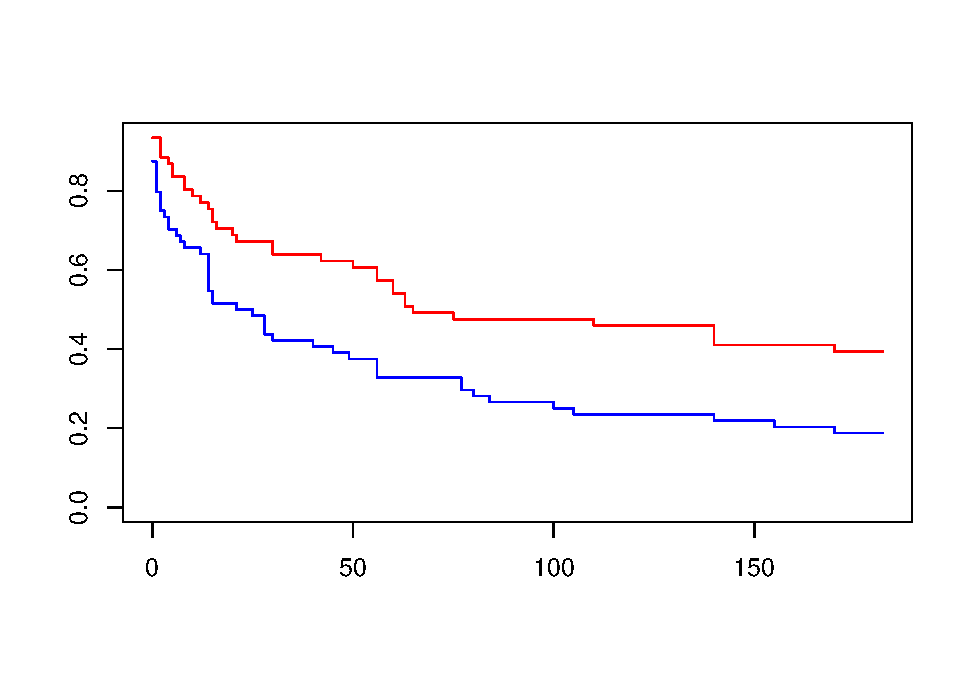
\includegraphics{hw_7_files/figure-latex/unnamed-chunk-1-1.pdf}

\begin{Shaded}
\begin{Highlighting}[]
\FunctionTok{table}\NormalTok{(pharmacoSmoking}\SpecialCharTok{$}\NormalTok{grp)}
\end{Highlighting}
\end{Shaded}

\begin{verbatim}
## 
## combination   patchOnly 
##          61          64
\end{verbatim}

\begin{Shaded}
\begin{Highlighting}[]
\DecValTok{25}\SpecialCharTok{/}\DecValTok{61}
\end{Highlighting}
\end{Shaded}

\begin{verbatim}
## [1] 0.4098361
\end{verbatim}

\begin{Shaded}
\begin{Highlighting}[]
\FloatTok{0.409}\SpecialCharTok{\^{}}\NormalTok{(}\DecValTok{1}\SpecialCharTok{/}\FloatTok{0.7}\NormalTok{)}\SpecialCharTok{*}\DecValTok{270} \SpecialCharTok{+} \FloatTok{0.409}\SpecialCharTok{*}\DecValTok{270}
\end{Highlighting}
\end{Shaded}

\begin{verbatim}
## [1] 185.7105
\end{verbatim}

\begin{Shaded}
\begin{Highlighting}[]
\DecValTok{186}\SpecialCharTok{+}\DecValTok{270}
\end{Highlighting}
\end{Shaded}

\begin{verbatim}
## [1] 456
\end{verbatim}

\begin{enumerate}
\def\labelenumi{\alph{enumi}.}
\setcounter{enumi}{1}
\tightlist
\item
  use simulations to find the sample size for a Cox proportional hazards
  model that includes group and age (linear) as covariates with a hazard
  ratio of 0.7 for group and -0.02 for age. Patients will be accrued to
  the study uniformly over 90 days, then followed-up for an additional
  90 days, there will be no other censoring other than the study ending
  at 180 days.
\end{enumerate}

\hypertarget{need-99-patients-in-this-setup.}{%
\section{Need 99 patients in this
setup.}\label{need-99-patients-in-this-setup.}}

\begin{Shaded}
\begin{Highlighting}[]
\FunctionTok{library}\NormalTok{(dplyr)}
\end{Highlighting}
\end{Shaded}

\begin{verbatim}
## 
## Attaching package: 'dplyr'
\end{verbatim}

\begin{verbatim}
## The following objects are masked from 'package:stats':
## 
##     filter, lag
\end{verbatim}

\begin{verbatim}
## The following objects are masked from 'package:base':
## 
##     intersect, setdiff, setequal, union
\end{verbatim}

\begin{Shaded}
\begin{Highlighting}[]
\FunctionTok{library}\NormalTok{(survival)}
\NormalTok{smoke1 }\OtherTok{\textless{}{-}}\NormalTok{ pharmacoSmoking }\SpecialCharTok{\%\textgreater{}\%} 
  \FunctionTok{filter}\NormalTok{(grp }\SpecialCharTok{==} \StringTok{"combination"}\NormalTok{) }\SpecialCharTok{\%\textgreater{}\%} \FunctionTok{filter}\NormalTok{(}\SpecialCharTok{!}\NormalTok{(ttr }\SpecialCharTok{\textless{}} \DecValTok{180} \SpecialCharTok{\&}\NormalTok{ relapse }\SpecialCharTok{==} \DecValTok{0}\NormalTok{))}

\NormalTok{smoke1}\SpecialCharTok{$}\NormalTok{censor }\OtherTok{=} \FunctionTok{ifelse}\NormalTok{(smoke1}\SpecialCharTok{$}\NormalTok{ttr }\SpecialCharTok{\textgreater{}=} \DecValTok{180}\NormalTok{, }\DecValTok{1}\NormalTok{, }\DecValTok{0}\NormalTok{)}
\end{Highlighting}
\end{Shaded}

\begin{Shaded}
\begin{Highlighting}[]
\FunctionTok{survreg}\NormalTok{(}\FunctionTok{Surv}\NormalTok{(ttr}\FloatTok{+0.001}\NormalTok{, relapse)}\SpecialCharTok{\textasciitilde{}}\DecValTok{1}\NormalTok{, }
        \AttributeTok{data=}\NormalTok{smoke1)}
\end{Highlighting}
\end{Shaded}

\begin{verbatim}
## Call:
## survreg(formula = Surv(ttr + 0.001, relapse) ~ 1, data = smoke1)
## 
## Coefficients:
## (Intercept) 
##    5.440526 
## 
## Scale= 2.51874 
## 
## Loglik(model)= -197.5   Loglik(intercept only)= -197.5
## n= 61
\end{verbatim}

\begin{Shaded}
\begin{Highlighting}[]
\NormalTok{simfun3 }\OtherTok{\textless{}{-}} \ControlFlowTok{function}\NormalTok{(}\AttributeTok{n=}\DecValTok{100}\NormalTok{, }\AttributeTok{beta\_t=} \FunctionTok{log}\NormalTok{(}\FloatTok{0.7}\NormalTok{),}
                    \AttributeTok{beta\_a=}\SpecialCharTok{{-}}\FloatTok{0.02}\NormalTok{,}
                    \AttributeTok{beta0=}\FunctionTok{log}\NormalTok{(}\FloatTok{5.27}\NormalTok{), }\AttributeTok{scale=}\FloatTok{1.93}\NormalTok{,}
                    \AttributeTok{accrual=}\DecValTok{90}\NormalTok{, }\AttributeTok{followup=}\DecValTok{90}\NormalTok{) \{}
\NormalTok{  age }\OtherTok{\textless{}{-}} \FunctionTok{sample}\NormalTok{(}\DecValTok{41}\SpecialCharTok{:}\DecValTok{56}\NormalTok{, n, }\AttributeTok{replace=}\ConstantTok{TRUE}\NormalTok{)}
\NormalTok{  treat }\OtherTok{\textless{}{-}} \FunctionTok{rep}\NormalTok{(}\DecValTok{0}\SpecialCharTok{:}\DecValTok{1}\NormalTok{, }\AttributeTok{each=}\NormalTok{n}\SpecialCharTok{/}\DecValTok{2}\NormalTok{)}
\NormalTok{  eta }\OtherTok{\textless{}{-}} \FunctionTok{exp}\NormalTok{(beta0 }\SpecialCharTok{+}\NormalTok{ beta\_t}\SpecialCharTok{*}\NormalTok{treat }\SpecialCharTok{+} 
\NormalTok{               beta\_a}\SpecialCharTok{*}\NormalTok{(age}\DecValTok{{-}41}\NormalTok{))}

\NormalTok{  time }\OtherTok{\textless{}{-}} \FunctionTok{rweibull}\NormalTok{(n, scale, eta)}
\NormalTok{  cens }\OtherTok{\textless{}{-}}\NormalTok{  followup}
\NormalTok{  tmpdat }\OtherTok{=} \FunctionTok{data.frame}\NormalTok{(}\AttributeTok{time =} \FunctionTok{pmin}\NormalTok{(time,cens),}
             \AttributeTok{status=}\FunctionTok{as.numeric}\NormalTok{(time }\SpecialCharTok{\textless{}}\NormalTok{ cens),}
             \AttributeTok{treat=}\NormalTok{treat,}
             \AttributeTok{age=}\NormalTok{age)}
\NormalTok{  fit1 }\OtherTok{=} \FunctionTok{coxph}\NormalTok{(}\FunctionTok{Surv}\NormalTok{(time,status) }\SpecialCharTok{\textasciitilde{}}\NormalTok{ treat}\SpecialCharTok{+}\NormalTok{age,}
              \AttributeTok{data=}\NormalTok{tmpdat)}
  \FunctionTok{summary}\NormalTok{(fit1)}\SpecialCharTok{$}\NormalTok{coef[}\DecValTok{1}\NormalTok{,}\DecValTok{5}\NormalTok{]}
\NormalTok{\}}


\NormalTok{out2 }\OtherTok{=} \FunctionTok{mean}\NormalTok{(}\FunctionTok{replicate}\NormalTok{(}\DecValTok{1000}\NormalTok{, }\FunctionTok{simfun3}\NormalTok{(}\AttributeTok{n=}\DecValTok{100}\NormalTok{)) }\SpecialCharTok{\textless{}} \FloatTok{0.05}\NormalTok{)}
\NormalTok{out2}
\end{Highlighting}
\end{Shaded}

\begin{verbatim}
## [1] 0.917
\end{verbatim}

\begin{enumerate}
\def\labelenumi{\arabic{enumi}.}
\setcounter{enumi}{1}
\tightlist
\item
  Fit a Poisson approximation model/piecewise constant hazard model to
  the pharmacoSmoking data using only group as a predictor/covariate and
  using time intervals for the constant hazards of 0-15, 15-40, and
  40-182 days.
\end{enumerate}

\begin{Shaded}
\begin{Highlighting}[]
\NormalTok{phsmoke }\OtherTok{\textless{}{-}} \FunctionTok{survSplit}\NormalTok{( }\FunctionTok{Surv}\NormalTok{(}\FunctionTok{I}\NormalTok{(ttr}\FloatTok{+0.5}\NormalTok{), relapse)}\SpecialCharTok{\textasciitilde{}}\NormalTok{grp, }\AttributeTok{data=}\NormalTok{pharmacoSmoking,}
                         \AttributeTok{cut=}\FunctionTok{c}\NormalTok{(}\DecValTok{15}\NormalTok{,}\DecValTok{40}\NormalTok{),}
                         \AttributeTok{id=}\StringTok{"id"}\NormalTok{, }\AttributeTok{episode=}\StringTok{"timeblock"}\NormalTok{)}

\NormalTok{phsmoke}\SpecialCharTok{$}\NormalTok{exp }\OtherTok{\textless{}{-}}\NormalTok{ phsmoke}\SpecialCharTok{$}\NormalTok{tstop }\SpecialCharTok{{-}}\NormalTok{ phsmoke}\SpecialCharTok{$}\NormalTok{tstart}
\NormalTok{phsmoke}\SpecialCharTok{$}\NormalTok{timeblock }\OtherTok{=} \FunctionTok{as.factor}\NormalTok{(phsmoke}\SpecialCharTok{$}\NormalTok{timeblock)}

\NormalTok{fit.pois }\OtherTok{\textless{}{-}} \FunctionTok{glm}\NormalTok{(relapse }\SpecialCharTok{\textasciitilde{}} \DecValTok{0} \SpecialCharTok{+} \FunctionTok{factor}\NormalTok{(timeblock)  }\SpecialCharTok{+} 
                 \FunctionTok{offset}\NormalTok{(}\FunctionTok{log}\NormalTok{(exp)) }\SpecialCharTok{+}
\NormalTok{                  grp, }\AttributeTok{data=}\NormalTok{phsmoke,}
               \AttributeTok{family=}\NormalTok{poisson)}

\FunctionTok{summary}\NormalTok{(fit.pois)}
\end{Highlighting}
\end{Shaded}

\begin{verbatim}
## 
## Call:
## glm(formula = relapse ~ 0 + factor(timeblock) + offset(log(exp)) + 
##     grp, family = poisson, data = phsmoke)
## 
## Deviance Residuals: 
##     Min       1Q   Median       3Q      Max  
## -1.3659  -0.9928  -0.7631   1.0837   3.0943  
## 
## Coefficients:
##                    Estimate Std. Error z value Pr(>|z|)    
## factor(timeblock)1  -3.8434     0.2024 -18.988  < 2e-16 ***
## factor(timeblock)2  -5.0911     0.2871 -17.731  < 2e-16 ***
## factor(timeblock)3  -5.6670     0.2150 -26.363  < 2e-16 ***
## grppatchOnly         0.6383     0.2160   2.955  0.00312 ** 
## ---
## Signif. codes:  0 '***' 0.001 '**' 0.01 '*' 0.05 '.' 0.1 ' ' 1
## 
## (Dispersion parameter for poisson family taken to be 1)
## 
##     Null deviance: 18974.59  on 272  degrees of freedom
## Residual deviance:   432.19  on 268  degrees of freedom
## AIC: 618.19
## 
## Number of Fisher Scoring iterations: 7
\end{verbatim}

\hypertarget{section-1}{%
\section{3)}\label{section-1}}

Fit a predictive model to the pharmacoSmoking data using all of the
covariates other than ageGroup2 and ageGroup4 (only linear terms for the
numerical covariates). Use the lasso with cross validation to find a
simpler predictive model. Show how it compares in prediction to the full
model and explain your choice of the penalty.

\hypertarget{the-best-lambda-is-3.}{%
\section{The best lambda is 3.}\label{the-best-lambda-is-3.}}

\hypertarget{this-model-does-better-than-the-other}{%
\section{This model does better than the
other}\label{this-model-does-better-than-the-other}}

\begin{Shaded}
\begin{Highlighting}[]
\FunctionTok{library}\NormalTok{(survival)}
\FunctionTok{library}\NormalTok{(asaur)}
\FunctionTok{library}\NormalTok{(penalized)}
\end{Highlighting}
\end{Shaded}

\begin{verbatim}
## Warning: package 'penalized' was built under R version 4.1.3
\end{verbatim}

\begin{verbatim}
## Welcome to penalized. For extended examples, see vignette("penalized").
\end{verbatim}

\begin{Shaded}
\begin{Highlighting}[]
\NormalTok{fit\_3 }\OtherTok{=} \FunctionTok{coxph}\NormalTok{(}\FunctionTok{Surv}\NormalTok{(ttr, relapse) }\SpecialCharTok{\textasciitilde{}}\NormalTok{ age }\SpecialCharTok{+}\NormalTok{ gender }\SpecialCharTok{+}\NormalTok{ race }\SpecialCharTok{+}\NormalTok{ employment }\SpecialCharTok{+}\NormalTok{ yearsSmoking }\SpecialCharTok{+}\NormalTok{ levelSmoking }\SpecialCharTok{+}\NormalTok{ priorAttempts }\SpecialCharTok{+}\NormalTok{ longestNoSmoke, }\AttributeTok{data =}\NormalTok{ pharmacoSmoking)}

\FunctionTok{summary}\NormalTok{(fit\_3)}
\end{Highlighting}
\end{Shaded}

\begin{verbatim}
## Call:
## coxph(formula = Surv(ttr, relapse) ~ age + gender + race + employment + 
##     yearsSmoking + levelSmoking + priorAttempts + longestNoSmoke, 
##     data = pharmacoSmoking)
## 
##   n= 125, number of events= 89 
## 
##                         coef  exp(coef)   se(coef)      z Pr(>|z|)   
## age               -5.693e-02  9.447e-01  2.136e-02 -2.665   0.0077 **
## genderMale        -5.761e-03  9.943e-01  2.418e-01 -0.024   0.9810   
## racehispanic      -6.049e-01  5.461e-01  5.214e-01 -1.160   0.2460   
## raceother         -1.321e+00  2.668e-01  1.040e+00 -1.271   0.2038   
## racewhite         -3.464e-01  7.072e-01  2.549e-01 -1.359   0.1743   
## employmentother    7.395e-01  2.095e+00  2.873e-01  2.574   0.0101 * 
## employmentpt       6.700e-01  1.954e+00  3.469e-01  1.932   0.0534 . 
## yearsSmoking       2.305e-02  1.023e+00  2.008e-02  1.148   0.2509   
## levelSmokinglight -5.819e-02  9.435e-01  2.670e-01 -0.218   0.8275   
## priorAttempts      1.679e-04  1.000e+00  1.111e-03  0.151   0.8799   
## longestNoSmoke    -8.397e-05  9.999e-01  1.260e-04 -0.667   0.5051   
## ---
## Signif. codes:  0 '***' 0.001 '**' 0.01 '*' 0.05 '.' 0.1 ' ' 1
## 
##                   exp(coef) exp(-coef) lower .95 upper .95
## age                  0.9447     1.0586   0.90593    0.9851
## genderMale           0.9943     1.0058   0.61894    1.5972
## racehispanic         0.5461     1.8310   0.19657    1.5174
## raceother            0.2668     3.7487   0.03476    2.0473
## racewhite            0.7072     1.4139   0.42911    1.1657
## employmentother      2.0949     0.4774   1.19285    3.6791
## employmentpt         1.9542     0.5117   0.99020    3.8566
## yearsSmoking         1.0233     0.9772   0.98383    1.0644
## levelSmokinglight    0.9435     1.0599   0.55905    1.5922
## priorAttempts        1.0002     0.9998   0.99799    1.0023
## longestNoSmoke       0.9999     1.0001   0.99967    1.0002
## 
## Concordance= 0.646  (se = 0.03 )
## Likelihood ratio test= 19.77  on 11 df,   p=0.05
## Wald test            = 18.95  on 11 df,   p=0.06
## Score (logrank) test = 19.3  on 11 df,   p=0.06
\end{verbatim}

\begin{Shaded}
\begin{Highlighting}[]
\NormalTok{lambdas }\OtherTok{\textless{}{-}} \FunctionTok{c}\NormalTok{(}\FloatTok{0.25}\NormalTok{, }\FloatTok{0.5}\NormalTok{, }\FloatTok{0.75}\NormalTok{, }\DecValTok{1}\SpecialCharTok{:}\DecValTok{40}\NormalTok{)}

\NormalTok{lfit.cm }\OtherTok{\textless{}{-}} \FunctionTok{lapply}\NormalTok{(lambdas, }\ControlFlowTok{function}\NormalTok{(lambda) \{}
  \FunctionTok{penalized}\NormalTok{(}
    \FunctionTok{Surv}\NormalTok{(ttr, relapse) }\SpecialCharTok{\textasciitilde{}}\NormalTok{ age }\SpecialCharTok{+}\NormalTok{ gender }\SpecialCharTok{+}\NormalTok{ race }\SpecialCharTok{+} 
\NormalTok{      employment }\SpecialCharTok{+}\NormalTok{ yearsSmoking }\SpecialCharTok{+}\NormalTok{ levelSmoking }\SpecialCharTok{+} 
\NormalTok{      priorAttempts }\SpecialCharTok{+}\NormalTok{ longestNoSmoke, }
    \AttributeTok{standardize=}\ConstantTok{TRUE}\NormalTok{,}
    \AttributeTok{data =}\NormalTok{ pharmacoSmoking,}
    \AttributeTok{lambda1 =}\NormalTok{ lambda}
\NormalTok{  )}
\NormalTok{\})}
\end{Highlighting}
\end{Shaded}

\begin{verbatim}
## # nonzero coefficients: 13# nonzero coefficients: 13          # nonzero coefficients: 13          # nonzero coefficients: 13          # nonzero coefficients: 13          # nonzero coefficients: 13          # nonzero coefficients: 13          # nonzero coefficients: 13          # nonzero coefficients: 13          # nonzero coefficients: 13          # nonzero coefficients: 13          # nonzero coefficients: 13          # nonzero coefficients: 13          # nonzero coefficients: 13          # nonzero coefficients: 13          # nonzero coefficients: 13          # nonzero coefficients: 13          # nonzero coefficients: 13          # nonzero coefficients: 13          # nonzero coefficients: 13          # nonzero coefficients: 13          # nonzero coefficients: 13          # nonzero coefficients: 13          # nonzero coefficients: 13          # nonzero coefficients: 13          # nonzero coefficients: 13          # nonzero coefficients: 13          # nonzero coefficients: 13          # nonzero coefficients: 13          # nonzero coefficients: 13          # nonzero coefficients: 13          # nonzero coefficients: 13          # nonzero coefficients: 13          # nonzero coefficients: 13          # nonzero coefficients: 13          # nonzero coefficients: 13          # nonzero coefficients: 13          # nonzero coefficients: 13          # nonzero coefficients: 13          # nonzero coefficients: 13          # nonzero coefficients: 13          # nonzero coefficients: 13          # nonzero coefficients: 13          # nonzero coefficients: 13          # nonzero coefficients: 13          # nonzero coefficients: 13          # nonzero coefficients: 13          # nonzero coefficients: 13          # nonzero coefficients: 13          # nonzero coefficients: 13          # nonzero coefficients: 13          # nonzero coefficients: 13          # nonzero coefficients: 13          # nonzero coefficients: 13          # nonzero coefficients: 13          # nonzero coefficients: 12          # nonzero coefficients: 12          # nonzero coefficients: 12          # nonzero coefficients: 12          # nonzero coefficients: 12          # nonzero coefficients: 12          # nonzero coefficients: 12          # nonzero coefficients: 12          # nonzero coefficients: 12          # nonzero coefficients: 12          # nonzero coefficients: 12          # nonzero coefficients: 12          # nonzero coefficients: 12          # nonzero coefficients: 12          # nonzero coefficients: 12          # nonzero coefficients: 12          # nonzero coefficients: 12          # nonzero coefficients: 12          # nonzero coefficients: 12          # nonzero coefficients: 12          # nonzero coefficients: 12          # nonzero coefficients: 12          # nonzero coefficients: 12          # nonzero coefficients: 12          # nonzero coefficients: 12          # nonzero coefficients: 12          # nonzero coefficients: 12          # nonzero coefficients: 12          # nonzero coefficients: 12          # nonzero coefficients: 12          # nonzero coefficients: 12          # nonzero coefficients: 12          # nonzero coefficients: 12          # nonzero coefficients: 12          # nonzero coefficients: 12          # nonzero coefficients: 12          # nonzero coefficients: 12          # nonzero coefficients: 12          # nonzero coefficients: 12          # nonzero coefficients: 12          # nonzero coefficients: 12          # nonzero coefficients: 12          # nonzero coefficients: 12          # nonzero coefficients: 12          # nonzero coefficients: 12          # nonzero coefficients: 12          # nonzero coefficients: 12          # nonzero coefficients: 12          # nonzero coefficients: 12          # nonzero coefficients: 12          # nonzero coefficients: 12          # nonzero coefficients: 12          # nonzero coefficients: 12          # nonzero coefficients: 12          # nonzero coefficients: 12          # nonzero coefficients: 12          # nonzero coefficients: 12          # nonzero coefficients: 12          # nonzero coefficients: 12          # nonzero coefficients: 12          # nonzero coefficients: 12          # nonzero coefficients: 12          # nonzero coefficients: 12          # nonzero coefficients: 12          # nonzero coefficients: 12          # nonzero coefficients: 12          # nonzero coefficients: 12          # nonzero coefficients: 12          # nonzero coefficients: 12          # nonzero coefficients: 12          # nonzero coefficients: 12          # nonzero coefficients: 12          # nonzero coefficients: 12          # nonzero coefficients: 12          # nonzero coefficients: 12          # nonzero coefficients: 12          # nonzero coefficients: 12          # nonzero coefficients: 12          # nonzero coefficients: 12          # nonzero coefficients: 12          # nonzero coefficients: 12          # nonzero coefficients: 12          # nonzero coefficients: 12          # nonzero coefficients: 12          # nonzero coefficients: 12          # nonzero coefficients: 12          # nonzero coefficients: 12          # nonzero coefficients: 12          # nonzero coefficients: 12          # nonzero coefficients: 12          # nonzero coefficients: 12          # nonzero coefficients: 12          # nonzero coefficients: 12          # nonzero coefficients: 12          # nonzero coefficients: 12          # nonzero coefficients: 12          # nonzero coefficients: 12          # nonzero coefficients: 12          # nonzero coefficients: 12          # nonzero coefficients: 12          # nonzero coefficients: 12          # nonzero coefficients: 12          # nonzero coefficients: 12          # nonzero coefficients: 12          # nonzero coefficients: 12          # nonzero coefficients: 12          # nonzero coefficients: 12          # nonzero coefficients: 12          # nonzero coefficients: 12          # nonzero coefficients: 12          # nonzero coefficients: 12          # nonzero coefficients: 12          # nonzero coefficients: 12          # nonzero coefficients: 12          # nonzero coefficients: 12          # nonzero coefficients: 12          # nonzero coefficients: 12          # nonzero coefficients: 12          # nonzero coefficients: 12          # nonzero coefficients: 12          # nonzero coefficients: 12          # nonzero coefficients: 12          # nonzero coefficients: 12          # nonzero coefficients: 12          # nonzero coefficients: 12          # nonzero coefficients: 12          # nonzero coefficients: 12          # nonzero coefficients: 12          # nonzero coefficients: 12          # nonzero coefficients: 12          # nonzero coefficients: 12          # nonzero coefficients: 12          # nonzero coefficients: 12          # nonzero coefficients: 12          # nonzero coefficients: 12          # nonzero coefficients: 12          # nonzero coefficients: 12          # nonzero coefficients: 12          # nonzero coefficients: 12          # nonzero coefficients: 12          # nonzero coefficients: 12          # nonzero coefficients: 12          # nonzero coefficients: 12          # nonzero coefficients: 12          # nonzero coefficients: 12          # nonzero coefficients: 12          # nonzero coefficients: 12          # nonzero coefficients: 12          # nonzero coefficients: 12          # nonzero coefficients: 12          # nonzero coefficients: 12          # nonzero coefficients: 12          # nonzero coefficients: 12          # nonzero coefficients: 12          # nonzero coefficients: 12          # nonzero coefficients: 12          # nonzero coefficients: 12          # nonzero coefficients: 12          # nonzero coefficients: 12          # nonzero coefficients: 12          # nonzero coefficients: 12          # nonzero coefficients: 12          # nonzero coefficients: 12          # nonzero coefficients: 12          # nonzero coefficients: 12          # nonzero coefficients: 12          # nonzero coefficients: 12          # nonzero coefficients: 12          # nonzero coefficients: 12          # nonzero coefficients: 12          # nonzero coefficients: 12          # nonzero coefficients: 12          # nonzero coefficients: 12          # nonzero coefficients: 12          # nonzero coefficients: 12          # nonzero coefficients: 12          # nonzero coefficients: 12          # nonzero coefficients: 12          # nonzero coefficients: 12          # nonzero coefficients: 12          # nonzero coefficients: 12          # nonzero coefficients: 12          # nonzero coefficients: 12          # nonzero coefficients: 11          # nonzero coefficients: 11          # nonzero coefficients: 11          # nonzero coefficients: 11          # nonzero coefficients: 11          # nonzero coefficients: 11          
## # nonzero coefficients: 13# nonzero coefficients: 12          # nonzero coefficients: 13          # nonzero coefficients: 13          # nonzero coefficients: 13          # nonzero coefficients: 13          # nonzero coefficients: 13          # nonzero coefficients: 13          # nonzero coefficients: 13          # nonzero coefficients: 13          # nonzero coefficients: 13          # nonzero coefficients: 13          # nonzero coefficients: 13          # nonzero coefficients: 13          # nonzero coefficients: 13          # nonzero coefficients: 13          # nonzero coefficients: 13          # nonzero coefficients: 13          # nonzero coefficients: 13          # nonzero coefficients: 13          # nonzero coefficients: 13          # nonzero coefficients: 13          # nonzero coefficients: 13          # nonzero coefficients: 13          # nonzero coefficients: 13          # nonzero coefficients: 13          # nonzero coefficients: 12          # nonzero coefficients: 12          # nonzero coefficients: 12          # nonzero coefficients: 12          # nonzero coefficients: 12          # nonzero coefficients: 12          # nonzero coefficients: 12          # nonzero coefficients: 12          # nonzero coefficients: 12          # nonzero coefficients: 12          # nonzero coefficients: 12          # nonzero coefficients: 12          # nonzero coefficients: 12          # nonzero coefficients: 12          # nonzero coefficients: 12          # nonzero coefficients: 12          # nonzero coefficients: 12          # nonzero coefficients: 12          # nonzero coefficients: 12          # nonzero coefficients: 12          # nonzero coefficients: 12          # nonzero coefficients: 12          # nonzero coefficients: 12          # nonzero coefficients: 12          # nonzero coefficients: 12          # nonzero coefficients: 12          # nonzero coefficients: 12          # nonzero coefficients: 12          # nonzero coefficients: 12          # nonzero coefficients: 12          # nonzero coefficients: 12          # nonzero coefficients: 12          # nonzero coefficients: 12          # nonzero coefficients: 12          # nonzero coefficients: 12          # nonzero coefficients: 12          # nonzero coefficients: 12          # nonzero coefficients: 12          # nonzero coefficients: 12          # nonzero coefficients: 12          # nonzero coefficients: 12          # nonzero coefficients: 12          # nonzero coefficients: 12          # nonzero coefficients: 12          # nonzero coefficients: 12          # nonzero coefficients: 12          # nonzero coefficients: 12          # nonzero coefficients: 12          # nonzero coefficients: 12          # nonzero coefficients: 12          # nonzero coefficients: 12          # nonzero coefficients: 12          # nonzero coefficients: 12          # nonzero coefficients: 12          # nonzero coefficients: 12          # nonzero coefficients: 12          # nonzero coefficients: 12          # nonzero coefficients: 12          # nonzero coefficients: 12          # nonzero coefficients: 12          # nonzero coefficients: 12          # nonzero coefficients: 12          # nonzero coefficients: 12          # nonzero coefficients: 12          # nonzero coefficients: 12          # nonzero coefficients: 12          # nonzero coefficients: 12          # nonzero coefficients: 12          # nonzero coefficients: 12          # nonzero coefficients: 11          # nonzero coefficients: 11          # nonzero coefficients: 11          # nonzero coefficients: 11          # nonzero coefficients: 11          # nonzero coefficients: 11          
## # nonzero coefficients: 13# nonzero coefficients: 12          # nonzero coefficients: 13          # nonzero coefficients: 13          # nonzero coefficients: 13          # nonzero coefficients: 13          # nonzero coefficients: 13          # nonzero coefficients: 13          # nonzero coefficients: 12          # nonzero coefficients: 13          # nonzero coefficients: 13          # nonzero coefficients: 13          # nonzero coefficients: 13          # nonzero coefficients: 13          # nonzero coefficients: 13          # nonzero coefficients: 13          # nonzero coefficients: 13          # nonzero coefficients: 13          # nonzero coefficients: 12          # nonzero coefficients: 12          # nonzero coefficients: 12          # nonzero coefficients: 12          # nonzero coefficients: 12          # nonzero coefficients: 12          # nonzero coefficients: 12          # nonzero coefficients: 12          # nonzero coefficients: 12          # nonzero coefficients: 12          # nonzero coefficients: 12          # nonzero coefficients: 12          # nonzero coefficients: 12          # nonzero coefficients: 12          # nonzero coefficients: 12          # nonzero coefficients: 12          # nonzero coefficients: 12          # nonzero coefficients: 12          # nonzero coefficients: 12          # nonzero coefficients: 12          # nonzero coefficients: 12          # nonzero coefficients: 12          # nonzero coefficients: 12          # nonzero coefficients: 12          # nonzero coefficients: 12          # nonzero coefficients: 12          # nonzero coefficients: 12          # nonzero coefficients: 12          # nonzero coefficients: 12          # nonzero coefficients: 12          # nonzero coefficients: 12          # nonzero coefficients: 12          # nonzero coefficients: 12          # nonzero coefficients: 12          # nonzero coefficients: 12          # nonzero coefficients: 12          # nonzero coefficients: 12          # nonzero coefficients: 12          # nonzero coefficients: 12          # nonzero coefficients: 12          # nonzero coefficients: 12          # nonzero coefficients: 12          # nonzero coefficients: 12          # nonzero coefficients: 12          # nonzero coefficients: 12          # nonzero coefficients: 12          # nonzero coefficients: 12          # nonzero coefficients: 12          # nonzero coefficients: 12          # nonzero coefficients: 12          # nonzero coefficients: 12          # nonzero coefficients: 12          # nonzero coefficients: 12          # nonzero coefficients: 12          # nonzero coefficients: 12          # nonzero coefficients: 12          # nonzero coefficients: 12          # nonzero coefficients: 12          # nonzero coefficients: 12          # nonzero coefficients: 12          # nonzero coefficients: 12          # nonzero coefficients: 12          # nonzero coefficients: 11          # nonzero coefficients: 11          # nonzero coefficients: 11          # nonzero coefficients: 11          # nonzero coefficients: 11          # nonzero coefficients: 11          
## # nonzero coefficients: 13# nonzero coefficients: 12          # nonzero coefficients: 13          # nonzero coefficients: 13          # nonzero coefficients: 13          # nonzero coefficients: 13          # nonzero coefficients: 13          # nonzero coefficients: 13          # nonzero coefficients: 12          # nonzero coefficients: 13          # nonzero coefficients: 13          # nonzero coefficients: 13          # nonzero coefficients: 12          # nonzero coefficients: 13          # nonzero coefficients: 13          # nonzero coefficients: 12          # nonzero coefficients: 12          # nonzero coefficients: 12          # nonzero coefficients: 12          # nonzero coefficients: 12          # nonzero coefficients: 12          # nonzero coefficients: 12          # nonzero coefficients: 12          # nonzero coefficients: 12          # nonzero coefficients: 12          # nonzero coefficients: 12          # nonzero coefficients: 12          # nonzero coefficients: 12          # nonzero coefficients: 12          # nonzero coefficients: 12          # nonzero coefficients: 12          # nonzero coefficients: 12          # nonzero coefficients: 12          # nonzero coefficients: 12          # nonzero coefficients: 12          # nonzero coefficients: 12          # nonzero coefficients: 12          # nonzero coefficients: 12          # nonzero coefficients: 12          # nonzero coefficients: 12          # nonzero coefficients: 12          # nonzero coefficients: 12          # nonzero coefficients: 12          # nonzero coefficients: 12          # nonzero coefficients: 12          # nonzero coefficients: 12          # nonzero coefficients: 12          # nonzero coefficients: 12          # nonzero coefficients: 12          # nonzero coefficients: 12          # nonzero coefficients: 12          # nonzero coefficients: 12          # nonzero coefficients: 12          # nonzero coefficients: 11          # nonzero coefficients: 11          # nonzero coefficients: 11          # nonzero coefficients: 11          # nonzero coefficients: 11          # nonzero coefficients: 11          
## # nonzero coefficients: 13# nonzero coefficients: 11          # nonzero coefficients: 12          # nonzero coefficients: 12          # nonzero coefficients: 12          # nonzero coefficients: 11          # nonzero coefficients: 10          # nonzero coefficients: 11          # nonzero coefficients: 11          # nonzero coefficients: 11          # nonzero coefficients: 10          # nonzero coefficients: 10          # nonzero coefficients: 10          # nonzero coefficients: 10          # nonzero coefficients: 10          # nonzero coefficients: 10          # nonzero coefficients: 10          # nonzero coefficients: 10          # nonzero coefficients: 10          # nonzero coefficients: 9          # nonzero coefficients: 9          # nonzero coefficients: 9          # nonzero coefficients: 9          # nonzero coefficients: 9          # nonzero coefficients: 8          # nonzero coefficients: 8          # nonzero coefficients: 8          # nonzero coefficients: 8          # nonzero coefficients: 8          # nonzero coefficients: 8          
## # nonzero coefficients: 13# nonzero coefficients: 11          # nonzero coefficients: 12          # nonzero coefficients: 11          # nonzero coefficients: 10          # nonzero coefficients: 9          # nonzero coefficients: 8          # nonzero coefficients: 9          # nonzero coefficients: 9          # nonzero coefficients: 8          # nonzero coefficients: 10          # nonzero coefficients: 10          # nonzero coefficients: 9          # nonzero coefficients: 8          # nonzero coefficients: 7          # nonzero coefficients: 6          # nonzero coefficients: 13          # nonzero coefficients: 13          # nonzero coefficients: 13          # nonzero coefficients: 13          # nonzero coefficients: 13          # nonzero coefficients: 12          # nonzero coefficients: 11          # nonzero coefficients: 10          # nonzero coefficients: 10          # nonzero coefficients: 10          # nonzero coefficients: 9          # nonzero coefficients: 10          # nonzero coefficients: 10          # nonzero coefficients: 9          # nonzero coefficients: 9          # nonzero coefficients: 8          # nonzero coefficients: 8          # nonzero coefficients: 8          # nonzero coefficients: 8          # nonzero coefficients: 8          # nonzero coefficients: 7          # nonzero coefficients: 8          # nonzero coefficients: 8          # nonzero coefficients: 7          # nonzero coefficients: 7          # nonzero coefficients: 7          # nonzero coefficients: 7          # nonzero coefficients: 7          # nonzero coefficients: 6          # nonzero coefficients: 6          # nonzero coefficients: 6          # nonzero coefficients: 6          # nonzero coefficients: 6          
## # nonzero coefficients: 13# nonzero coefficients: 11          # nonzero coefficients: 11          # nonzero coefficients: 10          # nonzero coefficients: 9          # nonzero coefficients: 9          # nonzero coefficients: 8          # nonzero coefficients: 8          # nonzero coefficients: 8          # nonzero coefficients: 8          # nonzero coefficients: 8          # nonzero coefficients: 7          # nonzero coefficients: 6          # nonzero coefficients: 6          # nonzero coefficients: 6          # nonzero coefficients: 6          # nonzero coefficients: 6          # nonzero coefficients: 6          
## # nonzero coefficients: 13# nonzero coefficients: 9          # nonzero coefficients: 10          # nonzero coefficients: 9          # nonzero coefficients: 8          # nonzero coefficients: 8          # nonzero coefficients: 7          # nonzero coefficients: 7          # nonzero coefficients: 8          # nonzero coefficients: 7          # nonzero coefficients: 6          # nonzero coefficients: 6          # nonzero coefficients: 6          # nonzero coefficients: 6          # nonzero coefficients: 6          # nonzero coefficients: 6          # nonzero coefficients: 6          
## # nonzero coefficients: 13# nonzero coefficients: 8          # nonzero coefficients: 9          # nonzero coefficients: 8          # nonzero coefficients: 8          # nonzero coefficients: 7          # nonzero coefficients: 6          # nonzero coefficients: 5          # nonzero coefficients: 5          # nonzero coefficients: 5          # nonzero coefficients: 5          # nonzero coefficients: 5          # nonzero coefficients: 5          
## # nonzero coefficients: 13# nonzero coefficients: 8          # nonzero coefficients: 9          # nonzero coefficients: 8          # nonzero coefficients: 7          # nonzero coefficients: 6          # nonzero coefficients: 5          # nonzero coefficients: 5          # nonzero coefficients: 5          # nonzero coefficients: 5          # nonzero coefficients: 5          # nonzero coefficients: 5          
## # nonzero coefficients: 13# nonzero coefficients: 8          # nonzero coefficients: 9          # nonzero coefficients: 8          # nonzero coefficients: 8          # nonzero coefficients: 7          # nonzero coefficients: 6          # nonzero coefficients: 5          # nonzero coefficients: 5          # nonzero coefficients: 5          # nonzero coefficients: 5          # nonzero coefficients: 5          # nonzero coefficients: 5          
## # nonzero coefficients: 13# nonzero coefficients: 7          # nonzero coefficients: 8          # nonzero coefficients: 8          # nonzero coefficients: 7          # nonzero coefficients: 6          # nonzero coefficients: 5          # nonzero coefficients: 5          # nonzero coefficients: 5          # nonzero coefficients: 5          # nonzero coefficients: 5          # nonzero coefficients: 5          
## # nonzero coefficients: 13# nonzero coefficients: 6          # nonzero coefficients: 6          # nonzero coefficients: 6          # nonzero coefficients: 5          # nonzero coefficients: 5          # nonzero coefficients: 5          # nonzero coefficients: 5          # nonzero coefficients: 5          # nonzero coefficients: 5          # nonzero coefficients: 5          
## # nonzero coefficients: 13# nonzero coefficients: 5          # nonzero coefficients: 5          # nonzero coefficients: 4          # nonzero coefficients: 3          # nonzero coefficients: 3          # nonzero coefficients: 3          # nonzero coefficients: 3          # nonzero coefficients: 3          # nonzero coefficients: 3          
## # nonzero coefficients: 13# nonzero coefficients: 3          # nonzero coefficients: 4          # nonzero coefficients: 3          # nonzero coefficients: 3          # nonzero coefficients: 3          # nonzero coefficients: 3          # nonzero coefficients: 3          # nonzero coefficients: 3          
## # nonzero coefficients: 13# nonzero coefficients: 3          # nonzero coefficients: 4          # nonzero coefficients: 3          # nonzero coefficients: 3          # nonzero coefficients: 3          # nonzero coefficients: 3          # nonzero coefficients: 3          # nonzero coefficients: 3          
## # nonzero coefficients: 13# nonzero coefficients: 3          # nonzero coefficients: 4          # nonzero coefficients: 3          # nonzero coefficients: 3          # nonzero coefficients: 2          # nonzero coefficients: 2          # nonzero coefficients: 2          # nonzero coefficients: 2          # nonzero coefficients: 2          # nonzero coefficients: 2          
## # nonzero coefficients: 13# nonzero coefficients: 3          # nonzero coefficients: 3          # nonzero coefficients: 2          # nonzero coefficients: 1          # nonzero coefficients: 2          # nonzero coefficients: 2          # nonzero coefficients: 2          # nonzero coefficients: 2          # nonzero coefficients: 2          # nonzero coefficients: 2          
## # nonzero coefficients: 13# nonzero coefficients: 2          # nonzero coefficients: 2          # nonzero coefficients: 1          # nonzero coefficients: 1          # nonzero coefficients: 1          # nonzero coefficients: 1          
## # nonzero coefficients: 13# nonzero coefficients: 1          # nonzero coefficients: 1          # nonzero coefficients: 1          # nonzero coefficients: 1          # nonzero coefficients: 1          
## # nonzero coefficients: 13# nonzero coefficients: 1          # nonzero coefficients: 1          # nonzero coefficients: 1          # nonzero coefficients: 1          # nonzero coefficients: 1          
## # nonzero coefficients: 13# nonzero coefficients: 1          # nonzero coefficients: 1          # nonzero coefficients: 1          # nonzero coefficients: 1          # nonzero coefficients: 1          
## # nonzero coefficients: 13# nonzero coefficients: 1          # nonzero coefficients: 1          # nonzero coefficients: 1          # nonzero coefficients: 1          
## # nonzero coefficients: 13# nonzero coefficients: 1          # nonzero coefficients: 1          # nonzero coefficients: 1          # nonzero coefficients: 1          
## # nonzero coefficients: 13# nonzero coefficients: 1          # nonzero coefficients: 1          # nonzero coefficients: 1          # nonzero coefficients: 1          
## # nonzero coefficients: 13# nonzero coefficients: 1          # nonzero coefficients: 1          # nonzero coefficients: 1          # nonzero coefficients: 1          
## # nonzero coefficients: 13# nonzero coefficients: 0          
## # nonzero coefficients: 13# nonzero coefficients: 0          
## # nonzero coefficients: 13# nonzero coefficients: 0          
## # nonzero coefficients: 13# nonzero coefficients: 0          
## # nonzero coefficients: 13# nonzero coefficients: 0          
## # nonzero coefficients: 13# nonzero coefficients: 0          
## # nonzero coefficients: 13# nonzero coefficients: 0          
## # nonzero coefficients: 13# nonzero coefficients: 0          
## # nonzero coefficients: 13# nonzero coefficients: 0          
## # nonzero coefficients: 13# nonzero coefficients: 0          
## # nonzero coefficients: 13# nonzero coefficients: 0          
## # nonzero coefficients: 13# nonzero coefficients: 0          
## # nonzero coefficients: 13# nonzero coefficients: 0          
## # nonzero coefficients: 13# nonzero coefficients: 0          
## # nonzero coefficients: 13# nonzero coefficients: 0          
## # nonzero coefficients: 13# nonzero coefficients: 0          
## # nonzero coefficients: 13# nonzero coefficients: 0          
\end{verbatim}

\begin{Shaded}
\begin{Highlighting}[]
\NormalTok{coef.cm }\OtherTok{\textless{}{-}} \FunctionTok{sapply}\NormalTok{(lfit.cm, coef, }\AttributeTok{which=}\StringTok{\textquotesingle{}all\textquotesingle{}}\NormalTok{) }\SpecialCharTok{|}\ErrorTok{\textgreater{}} 
  \FunctionTok{t}\NormalTok{() }

\FunctionTok{matplot}\NormalTok{(lambdas[}\SpecialCharTok{{-}}\DecValTok{1}\NormalTok{], coef.cm[}\SpecialCharTok{{-}}\DecValTok{1}\NormalTok{,], }\AttributeTok{type=}\StringTok{\textquotesingle{}l\textquotesingle{}}\NormalTok{, }\AttributeTok{lty=}\DecValTok{1}\NormalTok{, }\AttributeTok{col=}\DecValTok{1}\SpecialCharTok{:}\DecValTok{8}\NormalTok{)}
\FunctionTok{legend}\NormalTok{(}\StringTok{\textquotesingle{}bottomright\textquotesingle{}}\NormalTok{, }\AttributeTok{legend=}\FunctionTok{colnames}\NormalTok{(coef.cm), }\AttributeTok{lty=}\DecValTok{1}\NormalTok{, }\AttributeTok{col=}\DecValTok{1}\SpecialCharTok{:}\DecValTok{8}\NormalTok{)}
\end{Highlighting}
\end{Shaded}

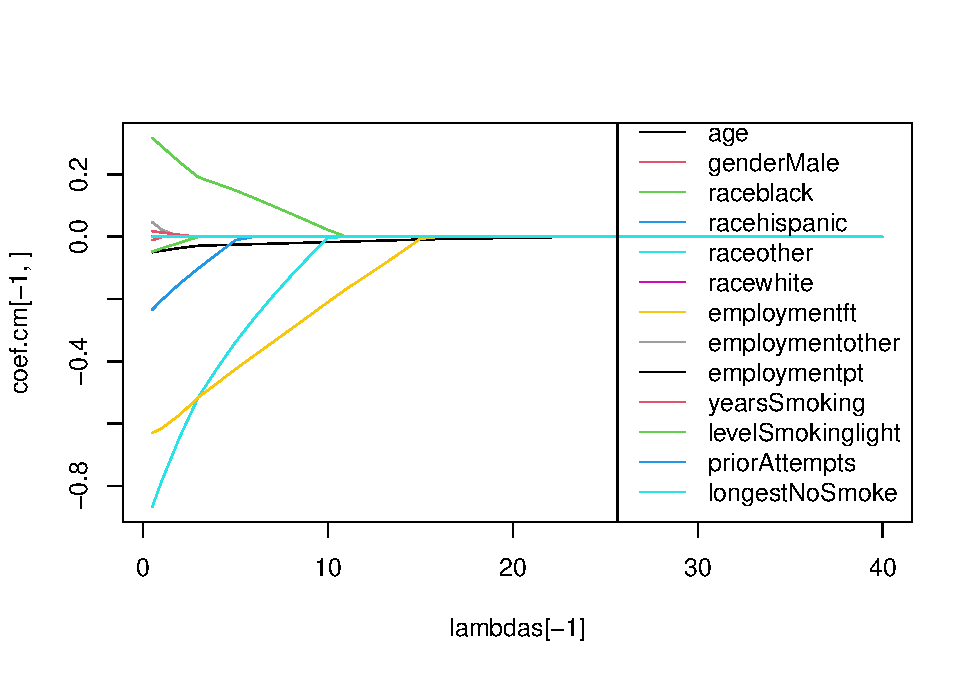
\includegraphics{hw_7_files/figure-latex/unnamed-chunk-5-1.pdf}

\begin{Shaded}
\begin{Highlighting}[]
\NormalTok{approx\_n }\OtherTok{\textless{}{-}} \FunctionTok{sapply}\NormalTok{(lfit.cm, }\ControlFlowTok{function}\NormalTok{(x) }\FunctionTok{sum}\NormalTok{(}\FunctionTok{coef}\NormalTok{(x)}\SpecialCharTok{!=}\DecValTok{0}\NormalTok{))}
\NormalTok{ll }\OtherTok{\textless{}{-}} \FunctionTok{sapply}\NormalTok{(lfit.cm, loglik)}
\NormalTok{aic }\OtherTok{\textless{}{-}} \SpecialCharTok{{-}}\NormalTok{ll }\SpecialCharTok{+} \DecValTok{2}\SpecialCharTok{*}\NormalTok{approx\_n}

\FunctionTok{plot}\NormalTok{(lambdas, aic)}
\end{Highlighting}
\end{Shaded}

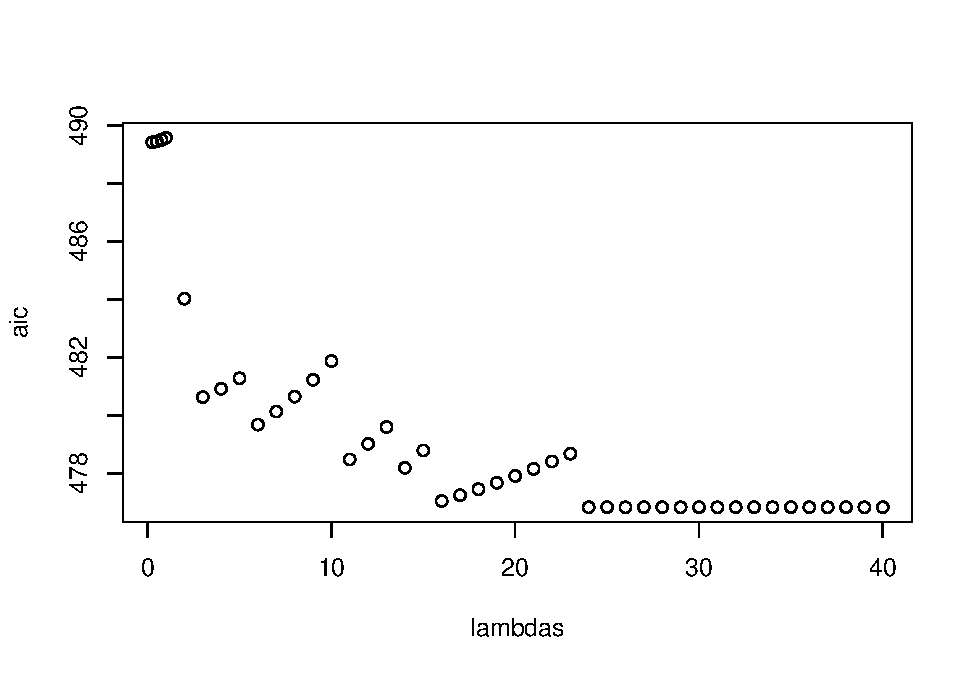
\includegraphics{hw_7_files/figure-latex/unnamed-chunk-5-2.pdf}

\begin{Shaded}
\begin{Highlighting}[]
\FunctionTok{set.seed}\NormalTok{(}\DecValTok{1}\NormalTok{)}
\NormalTok{folds }\OtherTok{\textless{}{-}} \FunctionTok{sample}\NormalTok{(}\FunctionTok{rep}\NormalTok{(}\DecValTok{1}\SpecialCharTok{:}\DecValTok{10}\NormalTok{, }\DecValTok{50}\NormalTok{))}

\NormalTok{cv.cm }\OtherTok{\textless{}{-}} \FunctionTok{lapply}\NormalTok{(lambdas[}\SpecialCharTok{{-}}\NormalTok{(}\DecValTok{1}\SpecialCharTok{:}\DecValTok{2}\NormalTok{)], }\ControlFlowTok{function}\NormalTok{(lambda) \{}
  \FunctionTok{cvl}\NormalTok{(}\FunctionTok{Surv}\NormalTok{(ttr, relapse) }\SpecialCharTok{\textasciitilde{}}\NormalTok{ age }\SpecialCharTok{+}\NormalTok{ gender }\SpecialCharTok{+}\NormalTok{ race }\SpecialCharTok{+} 
\NormalTok{      employment }\SpecialCharTok{+}\NormalTok{ yearsSmoking }\SpecialCharTok{+}\NormalTok{ levelSmoking }\SpecialCharTok{+} 
\NormalTok{      priorAttempts }\SpecialCharTok{+}\NormalTok{ longestNoSmoke, }
      \AttributeTok{data =}\NormalTok{ pharmacoSmoking,}
      \AttributeTok{lambda1 =}\NormalTok{ lambda, }
      \AttributeTok{fold =} \DecValTok{10}\NormalTok{)}
\NormalTok{\})}
\end{Highlighting}
\end{Shaded}

\begin{verbatim}
## 1234567891012345678910123456789101234567891012345678910123456789101234567891012345678910123456789101234567891012345678910123456789101234567891012345678910123456789101234567891012345678910123456789101234567891012345678910123456789101234567891012345678910123456789101234567891012345678910123456789101234567891012345678910123456789101234567891012345678910123456789101234567891012345678910123456789101234567891012345678910123456789101234567891012345678910
\end{verbatim}

\begin{Shaded}
\begin{Highlighting}[]
\NormalTok{cv.cm[[}\DecValTok{1}\NormalTok{]][[}\DecValTok{1}\NormalTok{]]}
\end{Highlighting}
\end{Shaded}

\begin{verbatim}
## [1] -501.4706
\end{verbatim}

\begin{Shaded}
\begin{Highlighting}[]
\NormalTok{lambdas[}\FunctionTok{which.max}\NormalTok{(}\FunctionTok{lapply}\NormalTok{(cv.cm, }\ControlFlowTok{function}\NormalTok{(x)\{x[[}\DecValTok{1}\NormalTok{]][[}\DecValTok{1}\NormalTok{]]\}))]}
\end{Highlighting}
\end{Shaded}

\begin{verbatim}
## [1] 1
\end{verbatim}

\begin{Shaded}
\begin{Highlighting}[]
\FunctionTok{plot}\NormalTok{(lambdas[}\SpecialCharTok{{-}}\FunctionTok{c}\NormalTok{(}\DecValTok{1}\NormalTok{,}\DecValTok{2}\NormalTok{)], }\FunctionTok{unlist}\NormalTok{(}\FunctionTok{lapply}\NormalTok{(cv.cm, }\ControlFlowTok{function}\NormalTok{(x)\{x[[}\DecValTok{1}\NormalTok{]][[}\DecValTok{1}\NormalTok{]]\})))}
\end{Highlighting}
\end{Shaded}

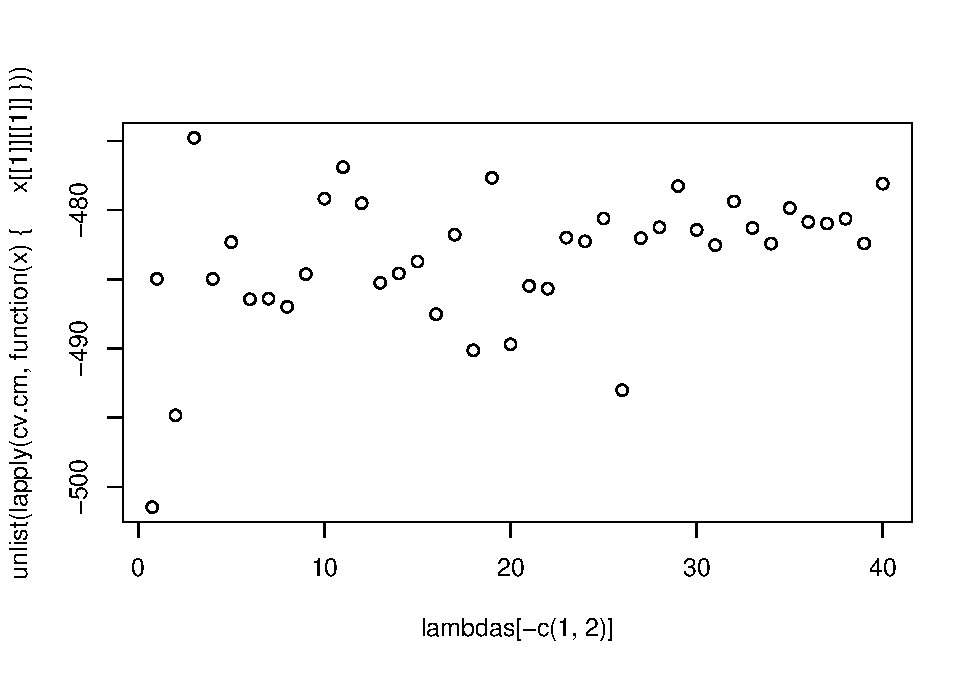
\includegraphics{hw_7_files/figure-latex/unnamed-chunk-5-3.pdf}

\begin{Shaded}
\begin{Highlighting}[]
\NormalTok{best\_lasso }\OtherTok{=} \FunctionTok{penalized}\NormalTok{(}
    \FunctionTok{Surv}\NormalTok{(ttr, relapse) }\SpecialCharTok{\textasciitilde{}}\NormalTok{ age }\SpecialCharTok{+}\NormalTok{ gender }\SpecialCharTok{+}\NormalTok{ race }\SpecialCharTok{+} 
\NormalTok{      employment }\SpecialCharTok{+}\NormalTok{ yearsSmoking }\SpecialCharTok{+}\NormalTok{ levelSmoking }\SpecialCharTok{+} 
\NormalTok{      priorAttempts }\SpecialCharTok{+}\NormalTok{ longestNoSmoke, }
    \AttributeTok{standardize=}\ConstantTok{TRUE}\NormalTok{,}
    \AttributeTok{data =}\NormalTok{ pharmacoSmoking,}
    \AttributeTok{lambda1 =} \DecValTok{3}
\NormalTok{  )}
\end{Highlighting}
\end{Shaded}

\begin{verbatim}
## # nonzero coefficients: 13# nonzero coefficients: 11          # nonzero coefficients: 12          # nonzero coefficients: 11          # nonzero coefficients: 10          # nonzero coefficients: 9          # nonzero coefficients: 8          # nonzero coefficients: 9          # nonzero coefficients: 9          # nonzero coefficients: 8          # nonzero coefficients: 10          # nonzero coefficients: 10          # nonzero coefficients: 9          # nonzero coefficients: 8          # nonzero coefficients: 7          # nonzero coefficients: 6          # nonzero coefficients: 13          # nonzero coefficients: 13          # nonzero coefficients: 13          # nonzero coefficients: 13          # nonzero coefficients: 13          # nonzero coefficients: 12          # nonzero coefficients: 11          # nonzero coefficients: 10          # nonzero coefficients: 10          # nonzero coefficients: 10          # nonzero coefficients: 9          # nonzero coefficients: 10          # nonzero coefficients: 10          # nonzero coefficients: 9          # nonzero coefficients: 9          # nonzero coefficients: 8          # nonzero coefficients: 8          # nonzero coefficients: 8          # nonzero coefficients: 8          # nonzero coefficients: 8          # nonzero coefficients: 7          # nonzero coefficients: 8          # nonzero coefficients: 8          # nonzero coefficients: 7          # nonzero coefficients: 7          # nonzero coefficients: 7          # nonzero coefficients: 7          # nonzero coefficients: 7          # nonzero coefficients: 6          # nonzero coefficients: 6          # nonzero coefficients: 6          # nonzero coefficients: 6          # nonzero coefficients: 6          
\end{verbatim}

\begin{Shaded}
\begin{Highlighting}[]
\CommentTok{\#predict(best\_lasso, newdata = pharmacoSmoking)}


\CommentTok{\# pen \textless{}{-} penalized(}
\CommentTok{\#         Surv(ttr, relapse), penalized = \textasciitilde{}age + gender + race + }
\CommentTok{\#       employment + yearsSmoking + levelSmoking + }
\CommentTok{\#       priorAttempts + longestNoSmoke, lambda1 = 3,}
\CommentTok{\#       unpenalized = Surv(ttr, relapse) \textasciitilde{} age + gender + race + }
\CommentTok{\#       employment + yearsSmoking + levelSmoking + }
\CommentTok{\#       priorAttempts + longestNoSmoke, data = pharmacoSmoking)}
\CommentTok{\# preds = predict(pen, data = pharmacoSmoking)}
\CommentTok{\# as.data.frame(preds) \%\textgreater{}\% View()}
\CommentTok{\# preds\_lasso = as.data.frame(preds)}
\CommentTok{\# plot(preds[,6])}
\CommentTok{\# plot(coxph(Surv(ttr, relapse) \textasciitilde{} age + gender + race + }
\CommentTok{\#       employment + yearsSmoking + levelSmoking + }
\CommentTok{\#       priorAttempts + longestNoSmoke, data = pharmacoSmoking))}
\CommentTok{\# preds = predict(fit\_3, newdata = pharmacoSmoking)}
\CommentTok{\# }
\CommentTok{\# plot(preds)}
\CommentTok{\# }
\CommentTok{\# predict(best\_lasso, data = pharmacoSmoking)}
\CommentTok{\# }
\CommentTok{\# mean((c(preds\_lasso[6,])*125 {-} pharmacoSmoking$ttr)\^{}2) \%\textgreater{}\% sqrt()}
\CommentTok{\# mean((preds*125 {-} pharmacoSmoking$ttr)\^{}2) \%\textgreater{}\% sqrt()}
\end{Highlighting}
\end{Shaded}

\hypertarget{section-2}{%
\section{4)}\label{section-2}}

The file ChildMort2.csv Download has data on child mortality. The
columns Age, Age.L, and Age.U have information on the interval censored
age at death. Using the interval censored data, estimate the survival
curve for the child mortality. Compare this curve to the standard
Kaplan-Meier estimate using the exit and event columns in the same
dataset.

\begin{Shaded}
\begin{Highlighting}[]
\CommentTok{\#install.packages("BiocManager")}

\FunctionTok{library}\NormalTok{(interval)}
\end{Highlighting}
\end{Shaded}

\begin{verbatim}
## Warning: package 'interval' was built under R version 4.1.3
\end{verbatim}

\begin{verbatim}
## Loading required package: perm
\end{verbatim}

\begin{verbatim}
## Warning: package 'perm' was built under R version 4.1.3
\end{verbatim}

\begin{verbatim}
## Loading required package: Icens
\end{verbatim}

\begin{verbatim}
## Loading required package: MLEcens
\end{verbatim}

\begin{verbatim}
## Warning: package 'MLEcens' was built under R version 4.1.3
\end{verbatim}

\begin{verbatim}
## Depends on Icens package available on bioconductor. 
## To install use for example:
## install.packages('BiocManager')
## BiocManager::install('Icens')
\end{verbatim}

\begin{Shaded}
\begin{Highlighting}[]
\NormalTok{child }\OtherTok{=} \FunctionTok{read.csv}\NormalTok{(}\StringTok{"ChildMort2.csv"}\NormalTok{)}
\FunctionTok{colnames}\NormalTok{(child)}
\end{Highlighting}
\end{Shaded}

\begin{verbatim}
## [1] "exit"  "event" "Age"   "Age.L" "Age.U"
\end{verbatim}

\begin{Shaded}
\begin{Highlighting}[]
\NormalTok{interval\_fit }\OtherTok{=} \FunctionTok{icfit}\NormalTok{(}\FunctionTok{Surv}\NormalTok{(Age.L, Age.U, }\AttributeTok{type=}\StringTok{\textquotesingle{}interval2\textquotesingle{}}\NormalTok{)}\SpecialCharTok{\textasciitilde{}}\DecValTok{1}\NormalTok{,}
             \AttributeTok{data=}\NormalTok{child)}

\FunctionTok{plot}\NormalTok{(interval\_fit, }\AttributeTok{ylim =} \FunctionTok{c}\NormalTok{(}\FloatTok{0.75}\NormalTok{,}\DecValTok{1}\NormalTok{))}
\FunctionTok{lines}\NormalTok{(}\FunctionTok{survfit}\NormalTok{(}\FunctionTok{Surv}\NormalTok{(exit, event)}\SpecialCharTok{\textasciitilde{}}\DecValTok{1}\NormalTok{, }\AttributeTok{data =}\NormalTok{ child), }\AttributeTok{col =} \StringTok{"red"}\NormalTok{)}
\end{Highlighting}
\end{Shaded}

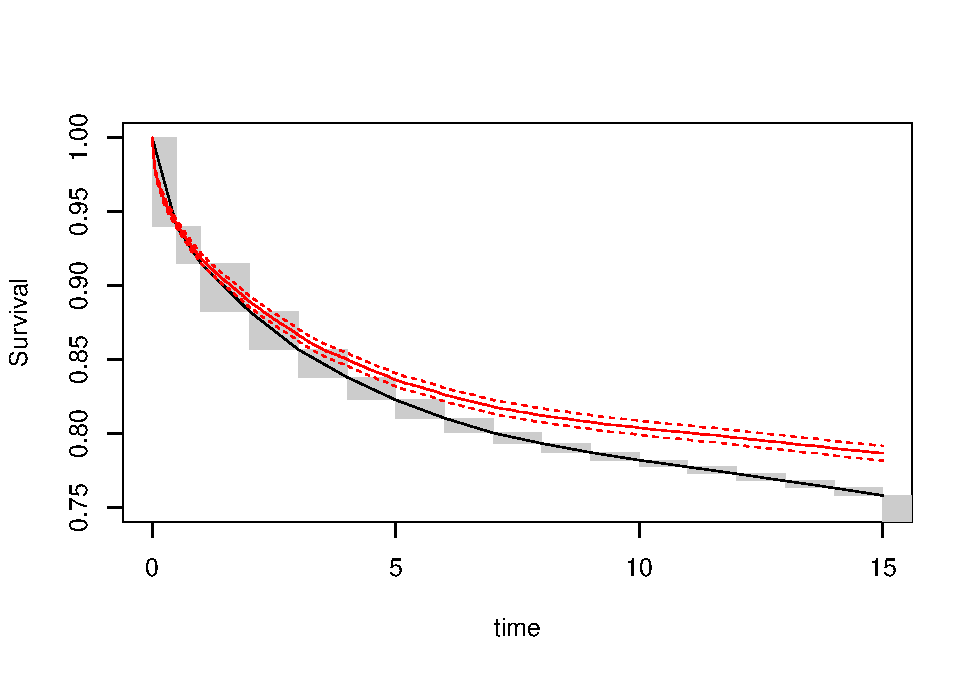
\includegraphics{hw_7_files/figure-latex/unnamed-chunk-7-1.pdf}

\end{document}
